\documentclass[twoside]{book}

% Packages required by doxygen
\usepackage{fixltx2e}
\usepackage{calc}
\usepackage{doxygen}
\usepackage[export]{adjustbox} % also loads graphicx
\usepackage{graphicx}
\usepackage[utf8]{inputenc}
\usepackage{makeidx}
\usepackage{multicol}
\usepackage{multirow}
\PassOptionsToPackage{warn}{textcomp}
\usepackage{textcomp}
\usepackage[nointegrals]{wasysym}
\usepackage[table]{xcolor}

% Font selection
\usepackage[T1]{fontenc}
\usepackage[scaled=.90]{helvet}
\usepackage{courier}
\usepackage{amssymb}
\usepackage{sectsty}
\renewcommand{\familydefault}{\sfdefault}
\allsectionsfont{%
  \fontseries{bc}\selectfont%
  \color{darkgray}%
}
\renewcommand{\DoxyLabelFont}{%
  \fontseries{bc}\selectfont%
  \color{darkgray}%
}
\newcommand{\+}{\discretionary{\mbox{\scriptsize$\hookleftarrow$}}{}{}}

% Page & text layout
\usepackage{geometry}
\geometry{%
  a4paper,%
  top=2.5cm,%
  bottom=2.5cm,%
  left=2.5cm,%
  right=2.5cm%
}
\tolerance=750
\hfuzz=15pt
\hbadness=750
\setlength{\emergencystretch}{15pt}
\setlength{\parindent}{0cm}
\setlength{\parskip}{3ex plus 2ex minus 2ex}
\makeatletter
\renewcommand{\paragraph}{%
  \@startsection{paragraph}{4}{0ex}{-1.0ex}{1.0ex}{%
    \normalfont\normalsize\bfseries\SS@parafont%
  }%
}
\renewcommand{\subparagraph}{%
  \@startsection{subparagraph}{5}{0ex}{-1.0ex}{1.0ex}{%
    \normalfont\normalsize\bfseries\SS@subparafont%
  }%
}
\makeatother

% Headers & footers
\usepackage{fancyhdr}
\pagestyle{fancyplain}
\fancyhead[LE]{\fancyplain{}{\bfseries\thepage}}
\fancyhead[CE]{\fancyplain{}{}}
\fancyhead[RE]{\fancyplain{}{\bfseries\leftmark}}
\fancyhead[LO]{\fancyplain{}{\bfseries\rightmark}}
\fancyhead[CO]{\fancyplain{}{}}
\fancyhead[RO]{\fancyplain{}{\bfseries\thepage}}
\fancyfoot[LE]{\fancyplain{}{}}
\fancyfoot[CE]{\fancyplain{}{}}
\fancyfoot[RE]{\fancyplain{}{\bfseries\scriptsize Generated by Doxygen }}
\fancyfoot[LO]{\fancyplain{}{\bfseries\scriptsize Generated by Doxygen }}
\fancyfoot[CO]{\fancyplain{}{}}
\fancyfoot[RO]{\fancyplain{}{}}
\renewcommand{\footrulewidth}{0.4pt}
\renewcommand{\chaptermark}[1]{%
  \markboth{#1}{}%
}
\renewcommand{\sectionmark}[1]{%
  \markright{\thesection\ #1}%
}

% Indices & bibliography
\usepackage{natbib}
\usepackage[titles]{tocloft}
\setcounter{tocdepth}{3}
\setcounter{secnumdepth}{5}
\makeindex

% Hyperlinks (required, but should be loaded last)
\usepackage{ifpdf}
\ifpdf
  \usepackage[pdftex,pagebackref=true]{hyperref}
\else
  \usepackage[ps2pdf,pagebackref=true]{hyperref}
\fi
\hypersetup{%
  colorlinks=true,%
  linkcolor=blue,%
  citecolor=blue,%
  unicode%
}

% Custom commands
\newcommand{\clearemptydoublepage}{%
  \newpage{\pagestyle{empty}\cleardoublepage}%
}

\usepackage{caption}
\captionsetup{labelsep=space,justification=centering,font={bf},singlelinecheck=off,skip=4pt,position=top}

%===== C O N T E N T S =====

\begin{document}

% Titlepage & ToC
\hypersetup{pageanchor=false,
             bookmarksnumbered=true,
             pdfencoding=unicode
            }
\pagenumbering{roman}
\begin{titlepage}
\vspace*{7cm}
\begin{center}%
{\Large My Project }\\
\vspace*{1cm}
{\large Generated by Doxygen 1.8.11}\\
\end{center}
\end{titlepage}
\clearemptydoublepage
\tableofcontents
\clearemptydoublepage
\pagenumbering{arabic}
\hypersetup{pageanchor=true}

%--- Begin generated contents ---
\chapter{termproject}
\label{md_README}
\hypertarget{md_README}{}
\input{md_README}
\chapter{Hierarchical Index}
\section{Class Hierarchy}
This inheritance list is sorted roughly, but not completely, alphabetically\+:\begin{DoxyCompactList}
\item \contentsline{section}{main\+\_\+savitch\+\_\+14\+:\+:game}{\pageref{classmain__savitch__14_1_1game}}{}
\begin{DoxyCompactList}
\item \contentsline{section}{main\+\_\+savitch\+\_\+14\+:\+:Othello}{\pageref{classmain__savitch__14_1_1Othello}}{}
\end{DoxyCompactList}
\item \contentsline{section}{main\+\_\+savitch\+\_\+14\+:\+:Piece}{\pageref{classmain__savitch__14_1_1Piece}}{}
\end{DoxyCompactList}

\chapter{Class Index}
\section{Class List}
Here are the classes, structs, unions and interfaces with brief descriptions\+:\begin{DoxyCompactList}
\item\contentsline{section}{\hyperlink{classmain__savitch__14_1_1game}{main\+\_\+savitch\+\_\+14\+::game} }{\pageref{classmain__savitch__14_1_1game}}{}
\item\contentsline{section}{\hyperlink{classmain__savitch__14_1_1Othello}{main\+\_\+savitch\+\_\+14\+::\+Othello} }{\pageref{classmain__savitch__14_1_1Othello}}{}
\item\contentsline{section}{\hyperlink{classmain__savitch__14_1_1Piece}{main\+\_\+savitch\+\_\+14\+::\+Piece} }{\pageref{classmain__savitch__14_1_1Piece}}{}
\end{DoxyCompactList}

\chapter{File Index}
\section{File List}
Here is a list of all documented files with brief descriptions\+:\begin{DoxyCompactList}
\item\contentsline{section}{{\bfseries colors.\+h} }{\pageref{colors_8h}}{}
\item\contentsline{section}{\hyperlink{game_8cc}{game.\+cc} \\*This is a file includes moves, winer and some other functions }{\pageref{game_8cc}}{}
\item\contentsline{section}{{\bfseries game.\+h} }{\pageref{game_8h}}{}
\item\contentsline{section}{\hyperlink{main_8cc}{main.\+cc} \\*This is the main function }{\pageref{main_8cc}}{}
\item\contentsline{section}{\hyperlink{othello_8cc}{othello.\+cc} \\*This is a file includes check\+\_\+move check game over and some other functions }{\pageref{othello_8cc}}{}
\item\contentsline{section}{{\bfseries othello.\+h} }{\pageref{othello_8h}}{}
\item\contentsline{section}{{\bfseries piece.\+h} }{\pageref{piece_8h}}{}
\end{DoxyCompactList}

\chapter{Class Documentation}
\hypertarget{classmain__savitch__14_1_1game}{}\section{main\+\_\+savitch\+\_\+14\+:\+:game Class Reference}
\label{classmain__savitch__14_1_1game}\index{main\+\_\+savitch\+\_\+14\+::game@{main\+\_\+savitch\+\_\+14\+::game}}


Inheritance diagram for main\+\_\+savitch\+\_\+14\+:\+:game\+:\nopagebreak
\begin{figure}[H]
\begin{center}
\leavevmode
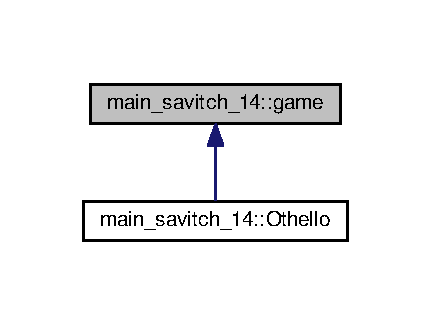
\includegraphics[width=207pt]{classmain__savitch__14_1_1game__inherit__graph}
\end{center}
\end{figure}
\subsection*{Public Types}
\begin{DoxyCompactItemize}
\item 
enum {\bfseries who} \{ {\bfseries H\+U\+M\+AN}, 
{\bfseries N\+E\+U\+T\+R\+AL}, 
{\bfseries C\+O\+M\+P\+U\+T\+ER}
 \}\hypertarget{classmain__savitch__14_1_1game_a4fe20fb287f809ae2b68e28e4ccba634}{}\label{classmain__savitch__14_1_1game_a4fe20fb287f809ae2b68e28e4ccba634}

\end{DoxyCompactItemize}
\subsection*{Public Member Functions}
\begin{DoxyCompactItemize}
\item 
who \hyperlink{classmain__savitch__14_1_1game_a96b7f20479c9c43bacc03b384467cba4}{play} (char level)
\end{DoxyCompactItemize}
\subsection*{Protected Member Functions}
\begin{DoxyCompactItemize}
\item 
virtual void \hyperlink{classmain__savitch__14_1_1game_ab8b87c3a1b68634861a8c0ed2b9f1992}{display\+\_\+message} (const std\+::string \&message) const 
\begin{DoxyCompactList}\small\item\em display message a message \end{DoxyCompactList}\item 
virtual std\+::string {\bfseries get\+\_\+user\+\_\+move} () const \hypertarget{classmain__savitch__14_1_1game_a1265f262f5a15bca5b532e6e97d13089}{}\label{classmain__savitch__14_1_1game_a1265f262f5a15bca5b532e6e97d13089}

\item 
virtual who {\bfseries last\+\_\+mover} () const \hypertarget{classmain__savitch__14_1_1game_a38d435da6aadc192ac10160b26ea0cc1}{}\label{classmain__savitch__14_1_1game_a38d435da6aadc192ac10160b26ea0cc1}

\item 
virtual int {\bfseries moves\+\_\+completed} () const \hypertarget{classmain__savitch__14_1_1game_aee677d1ef52c35474cb7c6071bb71749}{}\label{classmain__savitch__14_1_1game_aee677d1ef52c35474cb7c6071bb71749}

\item 
virtual who {\bfseries next\+\_\+mover} () const \hypertarget{classmain__savitch__14_1_1game_a0d445fdec3201c91c145ee2763e08922}{}\label{classmain__savitch__14_1_1game_a0d445fdec3201c91c145ee2763e08922}

\item 
virtual who {\bfseries opposite} (who player) const \hypertarget{classmain__savitch__14_1_1game_ae38d001e92ebe46e1a1433e41446c7ab}{}\label{classmain__savitch__14_1_1game_ae38d001e92ebe46e1a1433e41446c7ab}

\item 
virtual who \hyperlink{classmain__savitch__14_1_1game_a081611c42aa66b4d91bbefeec47c7c4e}{winning} () const 
\begin{DoxyCompactList}\small\item\em check who is the winner \end{DoxyCompactList}\item 
virtual void {\bfseries make\+\_\+move} (const std\+::string \&move)\hypertarget{classmain__savitch__14_1_1game_a20597d0caa907aea47b27fed8be3759b}{}\label{classmain__savitch__14_1_1game_a20597d0caa907aea47b27fed8be3759b}

\item 
virtual void {\bfseries restart} ()\hypertarget{classmain__savitch__14_1_1game_ad521a7d78e7c163a0bc28b709f0d45fd}{}\label{classmain__savitch__14_1_1game_ad521a7d78e7c163a0bc28b709f0d45fd}

\item 
virtual \hyperlink{classmain__savitch__14_1_1game}{game} $\ast$ {\bfseries clone} () const =0\hypertarget{classmain__savitch__14_1_1game_a7b663057f59210dd52738facfc40d959}{}\label{classmain__savitch__14_1_1game_a7b663057f59210dd52738facfc40d959}

\item 
virtual void {\bfseries compute\+\_\+moves} (std\+::queue$<$ std\+::string $>$ \&moves) const =0\hypertarget{classmain__savitch__14_1_1game_a2c0c049f5861026d0f639b5837889b7a}{}\label{classmain__savitch__14_1_1game_a2c0c049f5861026d0f639b5837889b7a}

\item 
virtual void {\bfseries display\+\_\+status} () const =0\hypertarget{classmain__savitch__14_1_1game_ac8205178922c49bab2865187e834b726}{}\label{classmain__savitch__14_1_1game_ac8205178922c49bab2865187e834b726}

\item 
virtual int {\bfseries evaluate} (char level) const =0\hypertarget{classmain__savitch__14_1_1game_a51429d44d3b51710fa8c9a34a8f2635e}{}\label{classmain__savitch__14_1_1game_a51429d44d3b51710fa8c9a34a8f2635e}

\item 
virtual bool {\bfseries is\+\_\+game\+\_\+over} () const =0\hypertarget{classmain__savitch__14_1_1game_a49eed20648918b03fd3e2cf78987b3d1}{}\label{classmain__savitch__14_1_1game_a49eed20648918b03fd3e2cf78987b3d1}

\item 
virtual bool {\bfseries is\+\_\+legal} (const std\+::string \&move) const =0\hypertarget{classmain__savitch__14_1_1game_ad38351422ca1ee3ae58440c1c6b36b30}{}\label{classmain__savitch__14_1_1game_ad38351422ca1ee3ae58440c1c6b36b30}

\end{DoxyCompactItemize}


\subsection{Member Function Documentation}
\index{main\+\_\+savitch\+\_\+14\+::game@{main\+\_\+savitch\+\_\+14\+::game}!display\+\_\+message@{display\+\_\+message}}
\index{display\+\_\+message@{display\+\_\+message}!main\+\_\+savitch\+\_\+14\+::game@{main\+\_\+savitch\+\_\+14\+::game}}
\subsubsection[{\texorpdfstring{display\+\_\+message(const std\+::string \&message) const }{display_message(const std::string &message) const }}]{\setlength{\rightskip}{0pt plus 5cm}void main\+\_\+savitch\+\_\+14\+::game\+::display\+\_\+message (
\begin{DoxyParamCaption}
\item[{const std\+::string \&}]{message}
\end{DoxyParamCaption}
) const\hspace{0.3cm}{\ttfamily [protected]}, {\ttfamily [virtual]}}\hypertarget{classmain__savitch__14_1_1game_ab8b87c3a1b68634861a8c0ed2b9f1992}{}\label{classmain__savitch__14_1_1game_ab8b87c3a1b68634861a8c0ed2b9f1992}


display message a message 


\begin{DoxyParams}{Parameters}
{\em message} & the message you want to display \\
\hline
\end{DoxyParams}


Reimplemented in \hyperlink{classmain__savitch__14_1_1Othello_a87ef083b9bc3943a0951f70c3ba9160a}{main\+\_\+savitch\+\_\+14\+::\+Othello}.

\index{main\+\_\+savitch\+\_\+14\+::game@{main\+\_\+savitch\+\_\+14\+::game}!play@{play}}
\index{play@{play}!main\+\_\+savitch\+\_\+14\+::game@{main\+\_\+savitch\+\_\+14\+::game}}
\subsubsection[{\texorpdfstring{play(char level)}{play(char level)}}]{\setlength{\rightskip}{0pt plus 5cm}game\+::who main\+\_\+savitch\+\_\+14\+::game\+::play (
\begin{DoxyParamCaption}
\item[{char}]{level}
\end{DoxyParamCaption}
)}\hypertarget{classmain__savitch__14_1_1game_a96b7f20479c9c43bacc03b384467cba4}{}\label{classmain__savitch__14_1_1game_a96b7f20479c9c43bacc03b384467cba4}
The play function should not be overridden. It plays one round of the game, with the human player moving first and the computer second. The return value is the winner of the game (or N\+E\+U\+T\+R\+AL for a tie). The commenting you see below sets this up for Phase One\index{main\+\_\+savitch\+\_\+14\+::game@{main\+\_\+savitch\+\_\+14\+::game}!winning@{winning}}
\index{winning@{winning}!main\+\_\+savitch\+\_\+14\+::game@{main\+\_\+savitch\+\_\+14\+::game}}
\subsubsection[{\texorpdfstring{winning() const }{winning() const }}]{\setlength{\rightskip}{0pt plus 5cm}game\+::who main\+\_\+savitch\+\_\+14\+::game\+::winning (
\begin{DoxyParamCaption}
{}
\end{DoxyParamCaption}
) const\hspace{0.3cm}{\ttfamily [protected]}, {\ttfamily [virtual]}}\hypertarget{classmain__savitch__14_1_1game_a081611c42aa66b4d91bbefeec47c7c4e}{}\label{classmain__savitch__14_1_1game_a081611c42aa66b4d91bbefeec47c7c4e}


check who is the winner 

\begin{DoxySeeAlso}{See also}
next\+\_\+mover() 

last\+\_\+mover() 
\end{DoxySeeAlso}


Reimplemented in \hyperlink{classmain__savitch__14_1_1Othello_a8934d1b63f73c03dae9629dbe03955d7}{main\+\_\+savitch\+\_\+14\+::\+Othello}.



The documentation for this class was generated from the following files\+:\begin{DoxyCompactItemize}
\item 
game.\+h\item 
\hyperlink{game_8cc}{game.\+cc}\end{DoxyCompactItemize}

\hypertarget{classmain__savitch__14_1_1Othello}{}\section{main\+\_\+savitch\+\_\+14\+:\+:Othello Class Reference}
\label{classmain__savitch__14_1_1Othello}\index{main\+\_\+savitch\+\_\+14\+::\+Othello@{main\+\_\+savitch\+\_\+14\+::\+Othello}}


Inheritance diagram for main\+\_\+savitch\+\_\+14\+:\+:Othello\+:\nopagebreak
\begin{figure}[H]
\begin{center}
\leavevmode
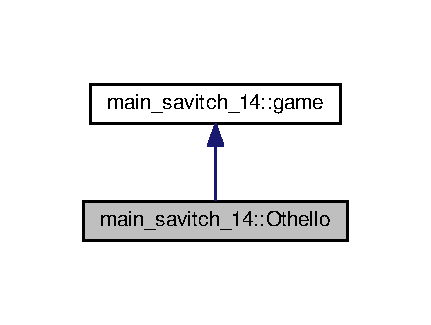
\includegraphics[width=207pt]{classmain__savitch__14_1_1Othello__inherit__graph}
\end{center}
\end{figure}


Collaboration diagram for main\+\_\+savitch\+\_\+14\+:\+:Othello\+:\nopagebreak
\begin{figure}[H]
\begin{center}
\leavevmode
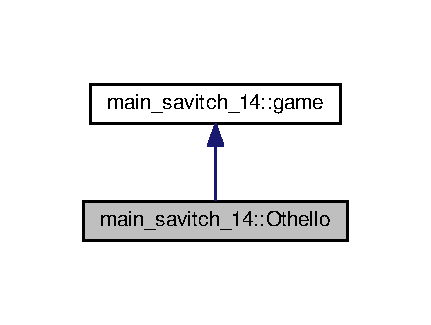
\includegraphics[width=207pt]{classmain__savitch__14_1_1Othello__coll__graph}
\end{center}
\end{figure}
\subsection*{Public Member Functions}
\begin{DoxyCompactItemize}
\item 
{\bfseries Othello} (const \hyperlink{classmain__savitch__14_1_1Othello}{Othello} \&other)\hypertarget{classmain__savitch__14_1_1Othello_a94d2c39352bca01e0896ef3a2fe94878}{}\label{classmain__savitch__14_1_1Othello_a94d2c39352bca01e0896ef3a2fe94878}

\item 
\hyperlink{classmain__savitch__14_1_1game}{game} $\ast$ {\bfseries clone} () const \hypertarget{classmain__savitch__14_1_1Othello_ac1f1e41b5acbc6bf7c0c41ea66a546be}{}\label{classmain__savitch__14_1_1Othello_ac1f1e41b5acbc6bf7c0c41ea66a546be}

\item 
void {\bfseries make\+\_\+move} (const std\+::string \&move)\hypertarget{classmain__savitch__14_1_1Othello_ac6aa8766ab2b905e6a9fe300f547e0c0}{}\label{classmain__savitch__14_1_1Othello_ac6aa8766ab2b905e6a9fe300f547e0c0}

\item 
void \hyperlink{classmain__savitch__14_1_1Othello_abf872b8074bfa4c04119317dc3b39af2}{restart} ()\hypertarget{classmain__savitch__14_1_1Othello_abf872b8074bfa4c04119317dc3b39af2}{}\label{classmain__savitch__14_1_1Othello_abf872b8074bfa4c04119317dc3b39af2}

\begin{DoxyCompactList}\small\item\em restart the game, set up four original locations \end{DoxyCompactList}\item 
void \hyperlink{classmain__savitch__14_1_1Othello_a471f0e8f0e63ed32d764682f60110267}{display\+\_\+status} () const 
\begin{DoxyCompactList}\small\item\em display current status \end{DoxyCompactList}\item 
bool \hyperlink{classmain__savitch__14_1_1Othello_af25b1502991e71e6bedbfa36a4006a8c}{is\+\_\+legal} (const std\+::string \&move) const 
\begin{DoxyCompactList}\small\item\em check if the location player choose is legal or not \end{DoxyCompactList}\item 
void \hyperlink{classmain__savitch__14_1_1Othello_a87ef083b9bc3943a0951f70c3ba9160a}{display\+\_\+message} (const std\+::string \&message) const 
\begin{DoxyCompactList}\small\item\em display the message for next step \end{DoxyCompactList}\item 
bool \hyperlink{classmain__savitch__14_1_1Othello_a4387d20f953aab54025760ec3f72f7ca}{is\+\_\+game\+\_\+over} () const 
\begin{DoxyCompactList}\small\item\em check if game is over \end{DoxyCompactList}\item 
void \hyperlink{classmain__savitch__14_1_1Othello_aae15562565348c574b8e4c0b7782d19f}{compute\+\_\+moves} (std\+::queue$<$ std\+::string $>$ \&moves) const 
\begin{DoxyCompactList}\small\item\em make computer move \end{DoxyCompactList}\item 
int \hyperlink{classmain__savitch__14_1_1Othello_aa5a29557cb041e963e53f077d7932e16}{evaluate} (char level) const 
\begin{DoxyCompactList}\small\item\em for AI the make sure different location has different value \end{DoxyCompactList}\item 
void \hyperlink{classmain__savitch__14_1_1Othello_a49ca2e53baf37714c14c59875c270dc4}{flip\+\_\+flip} (int a, int b, int c, int d)
\begin{DoxyCompactList}\small\item\em flip\+\_\+flip after someone make moves \end{DoxyCompactList}\item 
void \hyperlink{classmain__savitch__14_1_1Othello_aa471c56d1634172f92acdfcbe3faa363}{pass} (std\+::string move)
\begin{DoxyCompactList}\small\item\em check if someone can move next step move \end{DoxyCompactList}\item 
bool \hyperlink{classmain__savitch__14_1_1Othello_a23310eaa078cddaf0fd86303f2f191f4}{up\+\_\+legal} (int a, int b, int c, int d) const 
\begin{DoxyCompactList}\small\item\em check if up side is legal \end{DoxyCompactList}\item 
bool \hyperlink{classmain__savitch__14_1_1Othello_a1a6041ee29e5586ec07bdfef782731d0}{down\+\_\+legal} (int a, int b, int c, int d) const 
\begin{DoxyCompactList}\small\item\em check if down side is legal \end{DoxyCompactList}\item 
bool \hyperlink{classmain__savitch__14_1_1Othello_a50e871a1c0ceb803f3ffc4d4b2987062}{left\+\_\+legal} (int a, int b, int c, int d) const 
\begin{DoxyCompactList}\small\item\em check if left side is legal \end{DoxyCompactList}\item 
bool \hyperlink{classmain__savitch__14_1_1Othello_ac094aa06f0df5ef57b03e249f892428e}{right\+\_\+legal} (int a, int b, int c, int d) const 
\begin{DoxyCompactList}\small\item\em check if right side is legal \end{DoxyCompactList}\item 
bool \hyperlink{classmain__savitch__14_1_1Othello_a8ec6b317a873a919836c4be0534427b9}{left\+\_\+up\+\_\+legal} (int a, int b, int c, int d) const 
\begin{DoxyCompactList}\small\item\em check if left up side is legal \end{DoxyCompactList}\item 
bool \hyperlink{classmain__savitch__14_1_1Othello_ab7af6485f5dc762e92f0858c193e088b}{right\+\_\+up\+\_\+legal} (int a, int b, int c, int d) const 
\begin{DoxyCompactList}\small\item\em check if right up side is legal \end{DoxyCompactList}\item 
bool \hyperlink{classmain__savitch__14_1_1Othello_a161a5b2a574446e9cf16e66fab96234d}{left\+\_\+down\+\_\+legal} (int a, int b, int c, int d) const 
\begin{DoxyCompactList}\small\item\em check if left down side is legal \end{DoxyCompactList}\item 
bool \hyperlink{classmain__savitch__14_1_1Othello_a639b1780203d650877491fd69e63871a}{right\+\_\+down\+\_\+legal} (int a, int b, int c, int d) const 
\begin{DoxyCompactList}\small\item\em check if right down side is legal \end{DoxyCompactList}\item 
bool \hyperlink{classmain__savitch__14_1_1Othello_a015372a23879814a43aed9b4259f9834}{all\+\_\+legal} (int a, int b, int c, int d) const 
\begin{DoxyCompactList}\small\item\em combine all check sides \end{DoxyCompactList}\item 
bool {\bfseries human\+\_\+legal} () const \hypertarget{classmain__savitch__14_1_1Othello_ac1a0125fe3994e4c2d24b1440e775da7}{}\label{classmain__savitch__14_1_1Othello_ac1a0125fe3994e4c2d24b1440e775da7}

\item 
bool \hyperlink{classmain__savitch__14_1_1Othello_aa0a3222b954bf36dec6de48bdf17ebb7}{computer\+\_\+legal} () const 
\begin{DoxyCompactList}\small\item\em check computer step is legal \end{DoxyCompactList}\item 
who \hyperlink{classmain__savitch__14_1_1Othello_a8934d1b63f73c03dae9629dbe03955d7}{winning} () const 
\begin{DoxyCompactList}\small\item\em check who is the winnner \end{DoxyCompactList}\end{DoxyCompactItemize}
\subsection*{Additional Inherited Members}


\subsection{Member Function Documentation}
\index{main\+\_\+savitch\+\_\+14\+::\+Othello@{main\+\_\+savitch\+\_\+14\+::\+Othello}!all\+\_\+legal@{all\+\_\+legal}}
\index{all\+\_\+legal@{all\+\_\+legal}!main\+\_\+savitch\+\_\+14\+::\+Othello@{main\+\_\+savitch\+\_\+14\+::\+Othello}}
\subsubsection[{\texorpdfstring{all\+\_\+legal(int a, int b, int c, int d) const }{all_legal(int a, int b, int c, int d) const }}]{\setlength{\rightskip}{0pt plus 5cm}bool main\+\_\+savitch\+\_\+14\+::\+Othello\+::all\+\_\+legal (
\begin{DoxyParamCaption}
\item[{int}]{a, }
\item[{int}]{b, }
\item[{int}]{c, }
\item[{int}]{d}
\end{DoxyParamCaption}
) const}\hypertarget{classmain__savitch__14_1_1Othello_a015372a23879814a43aed9b4259f9834}{}\label{classmain__savitch__14_1_1Othello_a015372a23879814a43aed9b4259f9834}


combine all check sides 

\begin{DoxySeeAlso}{See also}
\hyperlink{classmain__savitch__14_1_1Othello_a23310eaa078cddaf0fd86303f2f191f4}{up\+\_\+legal()} 

\hyperlink{classmain__savitch__14_1_1Othello_a1a6041ee29e5586ec07bdfef782731d0}{down\+\_\+legal()} 

\hyperlink{classmain__savitch__14_1_1Othello_a50e871a1c0ceb803f3ffc4d4b2987062}{left\+\_\+legal()} 

\hyperlink{classmain__savitch__14_1_1Othello_ac094aa06f0df5ef57b03e249f892428e}{right\+\_\+legal()} 

\hyperlink{classmain__savitch__14_1_1Othello_a8ec6b317a873a919836c4be0534427b9}{left\+\_\+up\+\_\+legal()} 

\hyperlink{classmain__savitch__14_1_1Othello_ab7af6485f5dc762e92f0858c193e088b}{right\+\_\+up\+\_\+legal()} 

\hyperlink{classmain__savitch__14_1_1Othello_a161a5b2a574446e9cf16e66fab96234d}{left\+\_\+down\+\_\+legal()} 

\hyperlink{classmain__savitch__14_1_1Othello_a639b1780203d650877491fd69e63871a}{right\+\_\+down\+\_\+legal()} 

human\+\_\+legal() 

get\+\_\+piece() 

\hyperlink{classmain__savitch__14_1_1Othello_a015372a23879814a43aed9b4259f9834}{all\+\_\+legal()} 
\end{DoxySeeAlso}
\begin{DoxyReturn}{Returns}
return true if it is legal 
\end{DoxyReturn}
\index{main\+\_\+savitch\+\_\+14\+::\+Othello@{main\+\_\+savitch\+\_\+14\+::\+Othello}!compute\+\_\+moves@{compute\+\_\+moves}}
\index{compute\+\_\+moves@{compute\+\_\+moves}!main\+\_\+savitch\+\_\+14\+::\+Othello@{main\+\_\+savitch\+\_\+14\+::\+Othello}}
\subsubsection[{\texorpdfstring{compute\+\_\+moves(std\+::queue$<$ std\+::string $>$ \&moves) const }{compute_moves(std::queue< std::string > &moves) const }}]{\setlength{\rightskip}{0pt plus 5cm}void main\+\_\+savitch\+\_\+14\+::\+Othello\+::compute\+\_\+moves (
\begin{DoxyParamCaption}
\item[{std\+::queue$<$ std\+::string $>$ \&}]{moves}
\end{DoxyParamCaption}
) const\hspace{0.3cm}{\ttfamily [virtual]}}\hypertarget{classmain__savitch__14_1_1Othello_aae15562565348c574b8e4c0b7782d19f}{}\label{classmain__savitch__14_1_1Othello_aae15562565348c574b8e4c0b7782d19f}


make computer move 

\begin{DoxySeeAlso}{See also}
\hyperlink{classmain__savitch__14_1_1Othello_af25b1502991e71e6bedbfa36a4006a8c}{is\+\_\+legal()} 
\end{DoxySeeAlso}


Implements \hyperlink{classmain__savitch__14_1_1game}{main\+\_\+savitch\+\_\+14\+::game}.

\index{main\+\_\+savitch\+\_\+14\+::\+Othello@{main\+\_\+savitch\+\_\+14\+::\+Othello}!computer\+\_\+legal@{computer\+\_\+legal}}
\index{computer\+\_\+legal@{computer\+\_\+legal}!main\+\_\+savitch\+\_\+14\+::\+Othello@{main\+\_\+savitch\+\_\+14\+::\+Othello}}
\subsubsection[{\texorpdfstring{computer\+\_\+legal() const }{computer_legal() const }}]{\setlength{\rightskip}{0pt plus 5cm}bool main\+\_\+savitch\+\_\+14\+::\+Othello\+::computer\+\_\+legal (
\begin{DoxyParamCaption}
{}
\end{DoxyParamCaption}
) const}\hypertarget{classmain__savitch__14_1_1Othello_aa0a3222b954bf36dec6de48bdf17ebb7}{}\label{classmain__savitch__14_1_1Othello_aa0a3222b954bf36dec6de48bdf17ebb7}


check computer step is legal 

\begin{DoxySeeAlso}{See also}
get\+\_\+piece() 

\hyperlink{classmain__savitch__14_1_1Othello_a015372a23879814a43aed9b4259f9834}{all\+\_\+legal()} 
\end{DoxySeeAlso}
\begin{DoxyReturn}{Returns}
return true if it is legal 
\end{DoxyReturn}
\index{main\+\_\+savitch\+\_\+14\+::\+Othello@{main\+\_\+savitch\+\_\+14\+::\+Othello}!display\+\_\+message@{display\+\_\+message}}
\index{display\+\_\+message@{display\+\_\+message}!main\+\_\+savitch\+\_\+14\+::\+Othello@{main\+\_\+savitch\+\_\+14\+::\+Othello}}
\subsubsection[{\texorpdfstring{display\+\_\+message(const std\+::string \&message) const }{display_message(const std::string &message) const }}]{\setlength{\rightskip}{0pt plus 5cm}void main\+\_\+savitch\+\_\+14\+::\+Othello\+::display\+\_\+message (
\begin{DoxyParamCaption}
\item[{const std\+::string \&}]{message}
\end{DoxyParamCaption}
) const\hspace{0.3cm}{\ttfamily [virtual]}}\hypertarget{classmain__savitch__14_1_1Othello_a87ef083b9bc3943a0951f70c3ba9160a}{}\label{classmain__savitch__14_1_1Othello_a87ef083b9bc3943a0951f70c3ba9160a}


display the message for next step 


\begin{DoxyParams}{Parameters}
{\em message} & it is used for checking if it is legal move \\
\hline
\end{DoxyParams}
\begin{DoxySeeAlso}{See also}
next\+\_\+move() 

\hyperlink{classmain__savitch__14_1_1Othello_a87ef083b9bc3943a0951f70c3ba9160a}{display\+\_\+message()} 
\end{DoxySeeAlso}


Reimplemented from \hyperlink{classmain__savitch__14_1_1game_ab8b87c3a1b68634861a8c0ed2b9f1992}{main\+\_\+savitch\+\_\+14\+::game}.

\index{main\+\_\+savitch\+\_\+14\+::\+Othello@{main\+\_\+savitch\+\_\+14\+::\+Othello}!display\+\_\+status@{display\+\_\+status}}
\index{display\+\_\+status@{display\+\_\+status}!main\+\_\+savitch\+\_\+14\+::\+Othello@{main\+\_\+savitch\+\_\+14\+::\+Othello}}
\subsubsection[{\texorpdfstring{display\+\_\+status() const }{display_status() const }}]{\setlength{\rightskip}{0pt plus 5cm}void main\+\_\+savitch\+\_\+14\+::\+Othello\+::display\+\_\+status (
\begin{DoxyParamCaption}
{}
\end{DoxyParamCaption}
) const\hspace{0.3cm}{\ttfamily [virtual]}}\hypertarget{classmain__savitch__14_1_1Othello_a471f0e8f0e63ed32d764682f60110267}{}\label{classmain__savitch__14_1_1Othello_a471f0e8f0e63ed32d764682f60110267}


display current status 

\begin{DoxySeeAlso}{See also}
is\+\_\+black() 

is\+\_\+white() 

is\+\_\+empty() 

\hyperlink{classmain__savitch__14_1_1Othello_a4387d20f953aab54025760ec3f72f7ca}{is\+\_\+game\+\_\+over()} 
\end{DoxySeeAlso}


Implements \hyperlink{classmain__savitch__14_1_1game}{main\+\_\+savitch\+\_\+14\+::game}.

\index{main\+\_\+savitch\+\_\+14\+::\+Othello@{main\+\_\+savitch\+\_\+14\+::\+Othello}!down\+\_\+legal@{down\+\_\+legal}}
\index{down\+\_\+legal@{down\+\_\+legal}!main\+\_\+savitch\+\_\+14\+::\+Othello@{main\+\_\+savitch\+\_\+14\+::\+Othello}}
\subsubsection[{\texorpdfstring{down\+\_\+legal(int a, int b, int c, int d) const }{down_legal(int a, int b, int c, int d) const }}]{\setlength{\rightskip}{0pt plus 5cm}bool main\+\_\+savitch\+\_\+14\+::\+Othello\+::down\+\_\+legal (
\begin{DoxyParamCaption}
\item[{int}]{a, }
\item[{int}]{b, }
\item[{int}]{c, }
\item[{int}]{d}
\end{DoxyParamCaption}
) const}\hypertarget{classmain__savitch__14_1_1Othello_a1a6041ee29e5586ec07bdfef782731d0}{}\label{classmain__savitch__14_1_1Othello_a1a6041ee29e5586ec07bdfef782731d0}


check if down side is legal 

\begin{DoxySeeAlso}{See also}
get\+\_\+piece() 
\end{DoxySeeAlso}
\begin{DoxyReturn}{Returns}
return true if it is legal 
\end{DoxyReturn}
\index{main\+\_\+savitch\+\_\+14\+::\+Othello@{main\+\_\+savitch\+\_\+14\+::\+Othello}!evaluate@{evaluate}}
\index{evaluate@{evaluate}!main\+\_\+savitch\+\_\+14\+::\+Othello@{main\+\_\+savitch\+\_\+14\+::\+Othello}}
\subsubsection[{\texorpdfstring{evaluate(char level) const }{evaluate(char level) const }}]{\setlength{\rightskip}{0pt plus 5cm}int main\+\_\+savitch\+\_\+14\+::\+Othello\+::evaluate (
\begin{DoxyParamCaption}
\item[{char}]{level}
\end{DoxyParamCaption}
) const\hspace{0.3cm}{\ttfamily [virtual]}}\hypertarget{classmain__savitch__14_1_1Othello_aa5a29557cb041e963e53f077d7932e16}{}\label{classmain__savitch__14_1_1Othello_aa5a29557cb041e963e53f077d7932e16}


for AI the make sure different location has different value 

\begin{DoxySeeAlso}{See also}
is\+\_\+black() 

is\+\_\+white() 
\end{DoxySeeAlso}
\begin{DoxyReturn}{Returns}
the total evalueta value to know which location the best choice 
\end{DoxyReturn}


Implements \hyperlink{classmain__savitch__14_1_1game}{main\+\_\+savitch\+\_\+14\+::game}.

\index{main\+\_\+savitch\+\_\+14\+::\+Othello@{main\+\_\+savitch\+\_\+14\+::\+Othello}!flip\+\_\+flip@{flip\+\_\+flip}}
\index{flip\+\_\+flip@{flip\+\_\+flip}!main\+\_\+savitch\+\_\+14\+::\+Othello@{main\+\_\+savitch\+\_\+14\+::\+Othello}}
\subsubsection[{\texorpdfstring{flip\+\_\+flip(int a, int b, int c, int d)}{flip_flip(int a, int b, int c, int d)}}]{\setlength{\rightskip}{0pt plus 5cm}void main\+\_\+savitch\+\_\+14\+::\+Othello\+::flip\+\_\+flip (
\begin{DoxyParamCaption}
\item[{int}]{a, }
\item[{int}]{b, }
\item[{int}]{c, }
\item[{int}]{d}
\end{DoxyParamCaption}
)}\hypertarget{classmain__savitch__14_1_1Othello_a49ca2e53baf37714c14c59875c270dc4}{}\label{classmain__savitch__14_1_1Othello_a49ca2e53baf37714c14c59875c270dc4}


flip\+\_\+flip after someone make moves 

\begin{DoxySeeAlso}{See also}
get\+\_\+piece() 

\hyperlink{classmain__savitch__14_1_1Othello_a23310eaa078cddaf0fd86303f2f191f4}{up\+\_\+legal()} 

\hyperlink{classmain__savitch__14_1_1Othello_a1a6041ee29e5586ec07bdfef782731d0}{down\+\_\+legal()} 

\hyperlink{classmain__savitch__14_1_1Othello_a50e871a1c0ceb803f3ffc4d4b2987062}{left\+\_\+legal()} 

\hyperlink{classmain__savitch__14_1_1Othello_ac094aa06f0df5ef57b03e249f892428e}{right\+\_\+legal()} 

\hyperlink{classmain__savitch__14_1_1Othello_a8ec6b317a873a919836c4be0534427b9}{left\+\_\+up\+\_\+legal()} 

\hyperlink{classmain__savitch__14_1_1Othello_ab7af6485f5dc762e92f0858c193e088b}{right\+\_\+up\+\_\+legal()} 

\hyperlink{classmain__savitch__14_1_1Othello_a161a5b2a574446e9cf16e66fab96234d}{left\+\_\+down\+\_\+legal()} 

\hyperlink{classmain__savitch__14_1_1Othello_a639b1780203d650877491fd69e63871a}{right\+\_\+down\+\_\+legal()} 
\end{DoxySeeAlso}
\index{main\+\_\+savitch\+\_\+14\+::\+Othello@{main\+\_\+savitch\+\_\+14\+::\+Othello}!is\+\_\+game\+\_\+over@{is\+\_\+game\+\_\+over}}
\index{is\+\_\+game\+\_\+over@{is\+\_\+game\+\_\+over}!main\+\_\+savitch\+\_\+14\+::\+Othello@{main\+\_\+savitch\+\_\+14\+::\+Othello}}
\subsubsection[{\texorpdfstring{is\+\_\+game\+\_\+over() const }{is_game_over() const }}]{\setlength{\rightskip}{0pt plus 5cm}bool main\+\_\+savitch\+\_\+14\+::\+Othello\+::is\+\_\+game\+\_\+over (
\begin{DoxyParamCaption}
{}
\end{DoxyParamCaption}
) const\hspace{0.3cm}{\ttfamily [virtual]}}\hypertarget{classmain__savitch__14_1_1Othello_a4387d20f953aab54025760ec3f72f7ca}{}\label{classmain__savitch__14_1_1Othello_a4387d20f953aab54025760ec3f72f7ca}


check if game is over 

\begin{DoxyReturn}{Returns}
return true if game is over 
\end{DoxyReturn}
\begin{DoxySeeAlso}{See also}
get\+\_\+piese() 

human\+\_\+legal() 

\hyperlink{classmain__savitch__14_1_1Othello_aa0a3222b954bf36dec6de48bdf17ebb7}{computer\+\_\+legal()} 
\end{DoxySeeAlso}
\begin{DoxyReturn}{Returns}
return true if the game is over 
\end{DoxyReturn}


Implements \hyperlink{classmain__savitch__14_1_1game}{main\+\_\+savitch\+\_\+14\+::game}.

\index{main\+\_\+savitch\+\_\+14\+::\+Othello@{main\+\_\+savitch\+\_\+14\+::\+Othello}!is\+\_\+legal@{is\+\_\+legal}}
\index{is\+\_\+legal@{is\+\_\+legal}!main\+\_\+savitch\+\_\+14\+::\+Othello@{main\+\_\+savitch\+\_\+14\+::\+Othello}}
\subsubsection[{\texorpdfstring{is\+\_\+legal(const std\+::string \&move) const }{is_legal(const std::string &move) const }}]{\setlength{\rightskip}{0pt plus 5cm}bool main\+\_\+savitch\+\_\+14\+::\+Othello\+::is\+\_\+legal (
\begin{DoxyParamCaption}
\item[{const std\+::string \&}]{move}
\end{DoxyParamCaption}
) const\hspace{0.3cm}{\ttfamily [virtual]}}\hypertarget{classmain__savitch__14_1_1Othello_af25b1502991e71e6bedbfa36a4006a8c}{}\label{classmain__savitch__14_1_1Othello_af25b1502991e71e6bedbfa36a4006a8c}


check if the location player choose is legal or not 


\begin{DoxyParams}{Parameters}
{\em move} & the location which player choose \\
\hline
\end{DoxyParams}
\begin{DoxySeeAlso}{See also}
next\+\_\+move() 

get\+\_\+piese() 

\hyperlink{classmain__savitch__14_1_1Othello_a015372a23879814a43aed9b4259f9834}{all\+\_\+legal()} 
\end{DoxySeeAlso}
\begin{DoxyReturn}{Returns}
return true if the move is legal otherwise false 
\end{DoxyReturn}


Implements \hyperlink{classmain__savitch__14_1_1game}{main\+\_\+savitch\+\_\+14\+::game}.

\index{main\+\_\+savitch\+\_\+14\+::\+Othello@{main\+\_\+savitch\+\_\+14\+::\+Othello}!left\+\_\+down\+\_\+legal@{left\+\_\+down\+\_\+legal}}
\index{left\+\_\+down\+\_\+legal@{left\+\_\+down\+\_\+legal}!main\+\_\+savitch\+\_\+14\+::\+Othello@{main\+\_\+savitch\+\_\+14\+::\+Othello}}
\subsubsection[{\texorpdfstring{left\+\_\+down\+\_\+legal(int a, int b, int c, int d) const }{left_down_legal(int a, int b, int c, int d) const }}]{\setlength{\rightskip}{0pt plus 5cm}bool main\+\_\+savitch\+\_\+14\+::\+Othello\+::left\+\_\+down\+\_\+legal (
\begin{DoxyParamCaption}
\item[{int}]{a, }
\item[{int}]{b, }
\item[{int}]{c, }
\item[{int}]{d}
\end{DoxyParamCaption}
) const}\hypertarget{classmain__savitch__14_1_1Othello_a161a5b2a574446e9cf16e66fab96234d}{}\label{classmain__savitch__14_1_1Othello_a161a5b2a574446e9cf16e66fab96234d}


check if left down side is legal 

\begin{DoxySeeAlso}{See also}
get\+\_\+piece() 
\end{DoxySeeAlso}
\begin{DoxyReturn}{Returns}
return true if it is legal 
\end{DoxyReturn}
\index{main\+\_\+savitch\+\_\+14\+::\+Othello@{main\+\_\+savitch\+\_\+14\+::\+Othello}!left\+\_\+legal@{left\+\_\+legal}}
\index{left\+\_\+legal@{left\+\_\+legal}!main\+\_\+savitch\+\_\+14\+::\+Othello@{main\+\_\+savitch\+\_\+14\+::\+Othello}}
\subsubsection[{\texorpdfstring{left\+\_\+legal(int a, int b, int c, int d) const }{left_legal(int a, int b, int c, int d) const }}]{\setlength{\rightskip}{0pt plus 5cm}bool main\+\_\+savitch\+\_\+14\+::\+Othello\+::left\+\_\+legal (
\begin{DoxyParamCaption}
\item[{int}]{a, }
\item[{int}]{b, }
\item[{int}]{c, }
\item[{int}]{d}
\end{DoxyParamCaption}
) const}\hypertarget{classmain__savitch__14_1_1Othello_a50e871a1c0ceb803f3ffc4d4b2987062}{}\label{classmain__savitch__14_1_1Othello_a50e871a1c0ceb803f3ffc4d4b2987062}


check if left side is legal 

\begin{DoxySeeAlso}{See also}
get\+\_\+piece() 
\end{DoxySeeAlso}
\begin{DoxyReturn}{Returns}
return true if it is legal 
\end{DoxyReturn}
\index{main\+\_\+savitch\+\_\+14\+::\+Othello@{main\+\_\+savitch\+\_\+14\+::\+Othello}!left\+\_\+up\+\_\+legal@{left\+\_\+up\+\_\+legal}}
\index{left\+\_\+up\+\_\+legal@{left\+\_\+up\+\_\+legal}!main\+\_\+savitch\+\_\+14\+::\+Othello@{main\+\_\+savitch\+\_\+14\+::\+Othello}}
\subsubsection[{\texorpdfstring{left\+\_\+up\+\_\+legal(int a, int b, int c, int d) const }{left_up_legal(int a, int b, int c, int d) const }}]{\setlength{\rightskip}{0pt plus 5cm}bool main\+\_\+savitch\+\_\+14\+::\+Othello\+::left\+\_\+up\+\_\+legal (
\begin{DoxyParamCaption}
\item[{int}]{a, }
\item[{int}]{b, }
\item[{int}]{c, }
\item[{int}]{d}
\end{DoxyParamCaption}
) const}\hypertarget{classmain__savitch__14_1_1Othello_a8ec6b317a873a919836c4be0534427b9}{}\label{classmain__savitch__14_1_1Othello_a8ec6b317a873a919836c4be0534427b9}


check if left up side is legal 

\begin{DoxySeeAlso}{See also}
get\+\_\+piece() 
\end{DoxySeeAlso}
\begin{DoxyReturn}{Returns}
return true if it is legal 
\end{DoxyReturn}
\index{main\+\_\+savitch\+\_\+14\+::\+Othello@{main\+\_\+savitch\+\_\+14\+::\+Othello}!pass@{pass}}
\index{pass@{pass}!main\+\_\+savitch\+\_\+14\+::\+Othello@{main\+\_\+savitch\+\_\+14\+::\+Othello}}
\subsubsection[{\texorpdfstring{pass(std\+::string move)}{pass(std::string move)}}]{\setlength{\rightskip}{0pt plus 5cm}void main\+\_\+savitch\+\_\+14\+::\+Othello\+::pass (
\begin{DoxyParamCaption}
\item[{std\+::string}]{move}
\end{DoxyParamCaption}
)}\hypertarget{classmain__savitch__14_1_1Othello_aa471c56d1634172f92acdfcbe3faa363}{}\label{classmain__savitch__14_1_1Othello_aa471c56d1634172f92acdfcbe3faa363}


check if someone can move next step move 

\begin{DoxySeeAlso}{See also}
\hyperlink{classmain__savitch__14_1_1Othello_a4387d20f953aab54025760ec3f72f7ca}{is\+\_\+game\+\_\+over()} 

make\+\_\+move() 

\hyperlink{classmain__savitch__14_1_1Othello_aa0a3222b954bf36dec6de48bdf17ebb7}{computer\+\_\+legal()} 

human\+\_\+legal() 
\end{DoxySeeAlso}
\index{main\+\_\+savitch\+\_\+14\+::\+Othello@{main\+\_\+savitch\+\_\+14\+::\+Othello}!right\+\_\+down\+\_\+legal@{right\+\_\+down\+\_\+legal}}
\index{right\+\_\+down\+\_\+legal@{right\+\_\+down\+\_\+legal}!main\+\_\+savitch\+\_\+14\+::\+Othello@{main\+\_\+savitch\+\_\+14\+::\+Othello}}
\subsubsection[{\texorpdfstring{right\+\_\+down\+\_\+legal(int a, int b, int c, int d) const }{right_down_legal(int a, int b, int c, int d) const }}]{\setlength{\rightskip}{0pt plus 5cm}bool main\+\_\+savitch\+\_\+14\+::\+Othello\+::right\+\_\+down\+\_\+legal (
\begin{DoxyParamCaption}
\item[{int}]{a, }
\item[{int}]{b, }
\item[{int}]{c, }
\item[{int}]{d}
\end{DoxyParamCaption}
) const}\hypertarget{classmain__savitch__14_1_1Othello_a639b1780203d650877491fd69e63871a}{}\label{classmain__savitch__14_1_1Othello_a639b1780203d650877491fd69e63871a}


check if right down side is legal 

\begin{DoxySeeAlso}{See also}
get\+\_\+piece() 
\end{DoxySeeAlso}
\begin{DoxyReturn}{Returns}
return true if it is legal 
\end{DoxyReturn}
\index{main\+\_\+savitch\+\_\+14\+::\+Othello@{main\+\_\+savitch\+\_\+14\+::\+Othello}!right\+\_\+legal@{right\+\_\+legal}}
\index{right\+\_\+legal@{right\+\_\+legal}!main\+\_\+savitch\+\_\+14\+::\+Othello@{main\+\_\+savitch\+\_\+14\+::\+Othello}}
\subsubsection[{\texorpdfstring{right\+\_\+legal(int a, int b, int c, int d) const }{right_legal(int a, int b, int c, int d) const }}]{\setlength{\rightskip}{0pt plus 5cm}bool main\+\_\+savitch\+\_\+14\+::\+Othello\+::right\+\_\+legal (
\begin{DoxyParamCaption}
\item[{int}]{a, }
\item[{int}]{b, }
\item[{int}]{c, }
\item[{int}]{d}
\end{DoxyParamCaption}
) const}\hypertarget{classmain__savitch__14_1_1Othello_ac094aa06f0df5ef57b03e249f892428e}{}\label{classmain__savitch__14_1_1Othello_ac094aa06f0df5ef57b03e249f892428e}


check if right side is legal 

\begin{DoxySeeAlso}{See also}
get\+\_\+piece() 
\end{DoxySeeAlso}
\begin{DoxyReturn}{Returns}
return true if it is legal 
\end{DoxyReturn}
\index{main\+\_\+savitch\+\_\+14\+::\+Othello@{main\+\_\+savitch\+\_\+14\+::\+Othello}!right\+\_\+up\+\_\+legal@{right\+\_\+up\+\_\+legal}}
\index{right\+\_\+up\+\_\+legal@{right\+\_\+up\+\_\+legal}!main\+\_\+savitch\+\_\+14\+::\+Othello@{main\+\_\+savitch\+\_\+14\+::\+Othello}}
\subsubsection[{\texorpdfstring{right\+\_\+up\+\_\+legal(int a, int b, int c, int d) const }{right_up_legal(int a, int b, int c, int d) const }}]{\setlength{\rightskip}{0pt plus 5cm}bool main\+\_\+savitch\+\_\+14\+::\+Othello\+::right\+\_\+up\+\_\+legal (
\begin{DoxyParamCaption}
\item[{int}]{a, }
\item[{int}]{b, }
\item[{int}]{c, }
\item[{int}]{d}
\end{DoxyParamCaption}
) const}\hypertarget{classmain__savitch__14_1_1Othello_ab7af6485f5dc762e92f0858c193e088b}{}\label{classmain__savitch__14_1_1Othello_ab7af6485f5dc762e92f0858c193e088b}


check if right up side is legal 

\begin{DoxySeeAlso}{See also}
get\+\_\+piece() 
\end{DoxySeeAlso}
\begin{DoxyReturn}{Returns}
return true if it is legal 
\end{DoxyReturn}
\index{main\+\_\+savitch\+\_\+14\+::\+Othello@{main\+\_\+savitch\+\_\+14\+::\+Othello}!up\+\_\+legal@{up\+\_\+legal}}
\index{up\+\_\+legal@{up\+\_\+legal}!main\+\_\+savitch\+\_\+14\+::\+Othello@{main\+\_\+savitch\+\_\+14\+::\+Othello}}
\subsubsection[{\texorpdfstring{up\+\_\+legal(int a, int b, int c, int d) const }{up_legal(int a, int b, int c, int d) const }}]{\setlength{\rightskip}{0pt plus 5cm}bool main\+\_\+savitch\+\_\+14\+::\+Othello\+::up\+\_\+legal (
\begin{DoxyParamCaption}
\item[{int}]{a, }
\item[{int}]{b, }
\item[{int}]{c, }
\item[{int}]{d}
\end{DoxyParamCaption}
) const}\hypertarget{classmain__savitch__14_1_1Othello_a23310eaa078cddaf0fd86303f2f191f4}{}\label{classmain__savitch__14_1_1Othello_a23310eaa078cddaf0fd86303f2f191f4}


check if up side is legal 

\begin{DoxySeeAlso}{See also}
get\+\_\+piece() 
\end{DoxySeeAlso}
\begin{DoxyReturn}{Returns}
return true if it is legal 
\end{DoxyReturn}
\index{main\+\_\+savitch\+\_\+14\+::\+Othello@{main\+\_\+savitch\+\_\+14\+::\+Othello}!winning@{winning}}
\index{winning@{winning}!main\+\_\+savitch\+\_\+14\+::\+Othello@{main\+\_\+savitch\+\_\+14\+::\+Othello}}
\subsubsection[{\texorpdfstring{winning() const }{winning() const }}]{\setlength{\rightskip}{0pt plus 5cm}game\+::who main\+\_\+savitch\+\_\+14\+::\+Othello\+::winning (
\begin{DoxyParamCaption}
{}
\end{DoxyParamCaption}
) const\hspace{0.3cm}{\ttfamily [virtual]}}\hypertarget{classmain__savitch__14_1_1Othello_a8934d1b63f73c03dae9629dbe03955d7}{}\label{classmain__savitch__14_1_1Othello_a8934d1b63f73c03dae9629dbe03955d7}


check who is the winnner 

\begin{DoxySeeAlso}{See also}
get\+\_\+piece() 
\end{DoxySeeAlso}
\begin{DoxyReturn}{Returns}
return who wins this game otherwise return neutral 
\end{DoxyReturn}


Reimplemented from \hyperlink{classmain__savitch__14_1_1game_a081611c42aa66b4d91bbefeec47c7c4e}{main\+\_\+savitch\+\_\+14\+::game}.



The documentation for this class was generated from the following files\+:\begin{DoxyCompactItemize}
\item 
othello.\+h\item 
\hyperlink{othello_8cc}{othello.\+cc}\end{DoxyCompactItemize}

\hypertarget{classmain__savitch__14_1_1Piece}{}\section{main\+\_\+savitch\+\_\+14\+:\+:Piece Class Reference}
\label{classmain__savitch__14_1_1Piece}\index{main\+\_\+savitch\+\_\+14\+::\+Piece@{main\+\_\+savitch\+\_\+14\+::\+Piece}}
\subsection*{Public Member Functions}
\begin{DoxyCompactItemize}
\item 
int {\bfseries get\+\_\+horizontal} ()\hypertarget{classmain__savitch__14_1_1Piece_adb5a5097b1a3a0750cfb052bd3a0215d}{}\label{classmain__savitch__14_1_1Piece_adb5a5097b1a3a0750cfb052bd3a0215d}

\item 
int {\bfseries get\+\_\+vertical} ()\hypertarget{classmain__savitch__14_1_1Piece_a3d1aee3f481e21ebcf937b740ef2cdea}{}\label{classmain__savitch__14_1_1Piece_a3d1aee3f481e21ebcf937b740ef2cdea}

\item 
int {\bfseries get\+\_\+piece} (int i, int j)\hypertarget{classmain__savitch__14_1_1Piece_a616d9f83e798305fb2eab2de39a9b754}{}\label{classmain__savitch__14_1_1Piece_a616d9f83e798305fb2eab2de39a9b754}

\item 
void {\bfseries flip} (int i, int j, int p)\hypertarget{classmain__savitch__14_1_1Piece_a5bc38e6d888b011a75a44db64dee5dc3}{}\label{classmain__savitch__14_1_1Piece_a5bc38e6d888b011a75a44db64dee5dc3}

\item 
bool {\bfseries is\+\_\+empty} (int i, int j)\hypertarget{classmain__savitch__14_1_1Piece_a7c0a48c1f5990600e4559dbb7df275a4}{}\label{classmain__savitch__14_1_1Piece_a7c0a48c1f5990600e4559dbb7df275a4}

\item 
bool {\bfseries is\+\_\+black} (int i, int j)\hypertarget{classmain__savitch__14_1_1Piece_a0c185e81febae5e7267b04a9e4b759a9}{}\label{classmain__savitch__14_1_1Piece_a0c185e81febae5e7267b04a9e4b759a9}

\item 
bool {\bfseries is\+\_\+white} (int i, int j)\hypertarget{classmain__savitch__14_1_1Piece_a30f37028531752fe3777793e4d7f9025}{}\label{classmain__savitch__14_1_1Piece_a30f37028531752fe3777793e4d7f9025}

\end{DoxyCompactItemize}


The documentation for this class was generated from the following file\+:\begin{DoxyCompactItemize}
\item 
piece.\+h\end{DoxyCompactItemize}

\chapter{File Documentation}
\hypertarget{game_8cc}{}\section{game.\+cc File Reference}
\label{game_8cc}\index{game.\+cc@{game.\+cc}}


This is a file includes moves, winer and some other functions.  


{\ttfamily \#include $<$cassert$>$}\\*
{\ttfamily \#include $<$climits$>$}\\*
{\ttfamily \#include $<$iostream$>$}\\*
{\ttfamily \#include $<$queue$>$}\\*
{\ttfamily \#include $<$string$>$}\\*
{\ttfamily \#include \char`\"{}game.\+h\char`\"{}}\\*
Include dependency graph for game.\+cc\+:\nopagebreak
\begin{figure}[H]
\begin{center}
\leavevmode
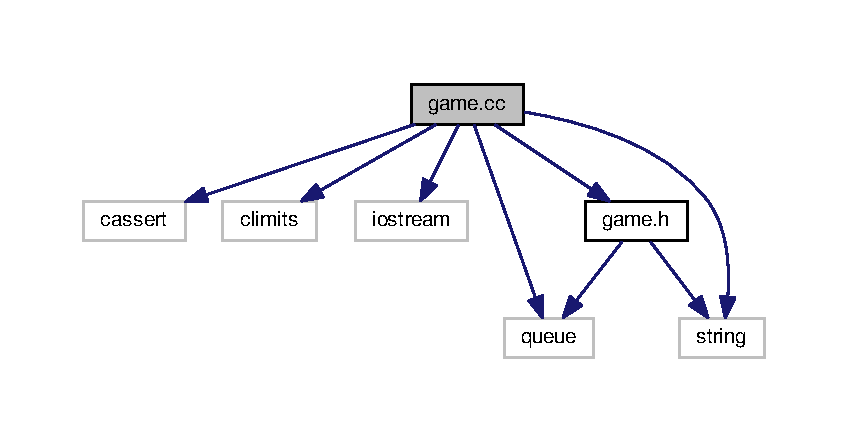
\includegraphics[width=350pt]{game_8cc__incl}
\end{center}
\end{figure}


\subsection{Detailed Description}
This is a file includes moves, winer and some other functions. 

\begin{DoxyAuthor}{Author}
Shipeng Yang, Zhaojie Chen, Bohong Li, Xudong Yuan 
\end{DoxyAuthor}
\begin{DoxyDate}{Date}
2017/11/12 
\end{DoxyDate}

\hypertarget{main_8cc}{}\section{main.\+cc File Reference}
\label{main_8cc}\index{main.\+cc@{main.\+cc}}


This is the main function.  


{\ttfamily \#include \char`\"{}game.\+h\char`\"{}}\\*
{\ttfamily \#include \char`\"{}othello.\+h\char`\"{}}\\*
{\ttfamily \#include $<$iostream$>$}\\*
Include dependency graph for main.\+cc\+:\nopagebreak
\begin{figure}[H]
\begin{center}
\leavevmode
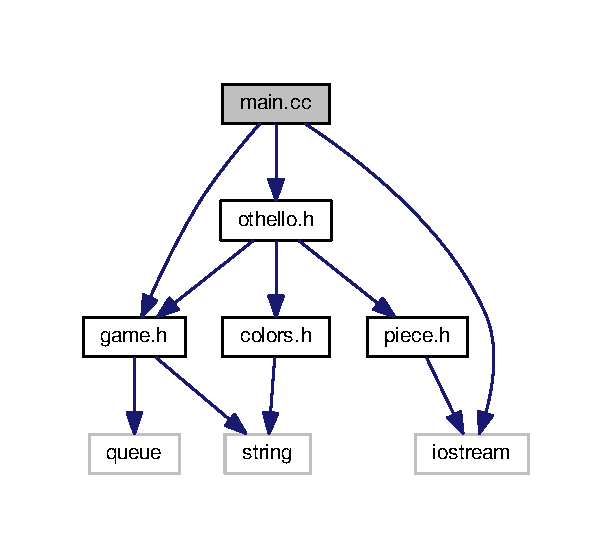
\includegraphics[width=294pt]{main_8cc__incl}
\end{center}
\end{figure}
\subsection*{Functions}
\begin{DoxyCompactItemize}
\item 
int {\bfseries main} ()\hypertarget{main_8cc_ae66f6b31b5ad750f1fe042a706a4e3d4}{}\label{main_8cc_ae66f6b31b5ad750f1fe042a706a4e3d4}

\end{DoxyCompactItemize}


\subsection{Detailed Description}
This is the main function. 

\begin{DoxyAuthor}{Author}
Shipeng Yang, Zhaojie Chen, Bohong Li, Xudong Yuan 
\end{DoxyAuthor}
\begin{DoxyDate}{Date}
2017/11/12 
\end{DoxyDate}

\hypertarget{othello_8cc}{}\section{othello.\+cc File Reference}
\label{othello_8cc}\index{othello.\+cc@{othello.\+cc}}


This is a file includes check\+\_\+move check game over and some other functions.  


{\ttfamily \#include \char`\"{}othello.\+h\char`\"{}}\\*
{\ttfamily \#include $<$iostream$>$}\\*
{\ttfamily \#include $<$stdio.\+h$>$}\\*
{\ttfamily \#include $<$queue$>$}\\*
Include dependency graph for othello.\+cc\+:\nopagebreak
\begin{figure}[H]
\begin{center}
\leavevmode
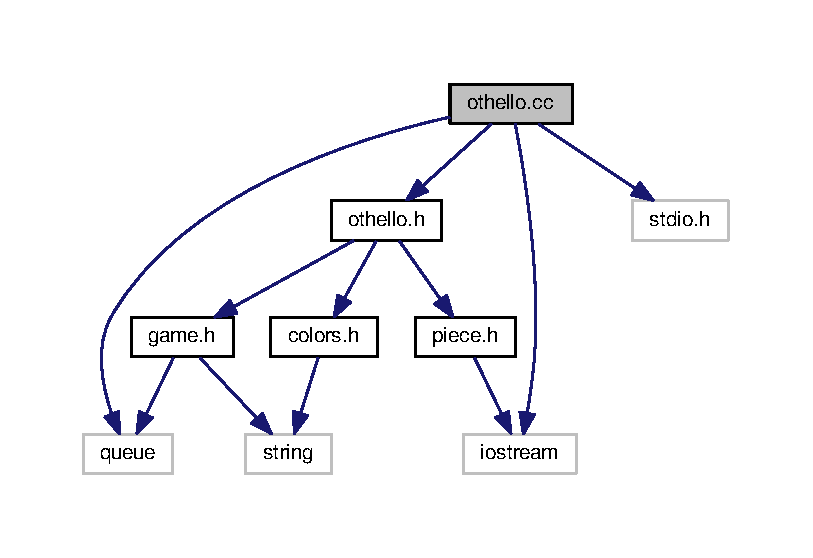
\includegraphics[width=350pt]{othello_8cc__incl}
\end{center}
\end{figure}


\subsection{Detailed Description}
This is a file includes check\+\_\+move check game over and some other functions. 

\begin{DoxyAuthor}{Author}
Shipeng Yang, Zhaojie Chen, Bohong Li, Xudong Yuan 
\end{DoxyAuthor}
\begin{DoxyDate}{Date}
2017/11/12 
\end{DoxyDate}

%--- End generated contents ---

% Index
\backmatter
\newpage
\phantomsection
\clearemptydoublepage
\addcontentsline{toc}{chapter}{Index}
\printindex

\end{document}
